\chapter{Alimentazione seriale}
%L'alimentazione seriale dei moduli è il sistema scelto per l'alimentazione, in grado di rispettare i requisiti per il nuovo tracciatore a pixel di fase due. 
\section{Introduzione}
Nel capitolo precedente si sono discussi i requisiti richiesti per il tracciatore di fase due: tolleranza agli alti livelli di radiazione, alta risoluzione, riduzione del materiale, etc... Per rispettare queste condizioni si è deciso di sviluppare un sistema di alimentazione innovativo e alternativo agli attuali convertitori DC-DC\footnote{L'attuale tracciatore utilizza un sistema di alimentazione in parallelo dei moduli, in cui i convertitori DC-DC generano localmente le tensioni necessarie al funzionamento del chip.}. 
Questi, infatti, non resisterebbero ai più alti livelli di radiazione della fase ad alta luminosità, nè sarebbero in grado di operare efficacemente in presenza del campo magnetico previsto.
Il nuovo sistema di alimentazione prevede una distribuzione seriale e sarà gestito, all'interno del chip, da circuiti dedicati prodotti in tecnologia CMOS a 65 nm.

%\section{Caratteristiche dell'alimentazione seriale}
In un sistema di alimentazione seriale il generatore fornisce tensione e corrente ad una catena di moduli posti in successione. 
A differenza del sistema di alimentazione parallelo attuale, in cui tutti i moduli si trovano allo stesso potenziale di riferimento e in cui la corrente totale erogata è la somma di quella che scorre nei singoli rami, nel sistema seriale attuale la corrente totale è la stessa che scorre in ciascun modulo ed è la tensione di lavoro a cambiare\footnote{La differenza di potenziale è la stessa per ciascun modulo, ma il riferimento di potenziale cambia per ciascuno di questi.}. 
Dato che la corrente viene ``riutilizzata'' in ciascun modulo, il generatore deve fornire correnti minori, rispetto a quelle di un sistema di alimentazione parallelo. Per questo motivo le perdite di potenza nei cavi sono ridotte ed è quindi posibile utilizzare cavi più sottili, riducendo il materiale presente all'interno del tracciatore.
%Questo significa che in ogni elemento scorre la medesima corrente, ma l'intervallo di tensione in cui viene a trovarsi è differente per ciascuno di essi. Fino ad ora il metodo di alimentazione utilizzato era quelo parallelo, tutti i moduli si trovano ad un potenziale comune ma su rami separati, questo implica che nel cavo principale scorre una corrente pari alla somma di quella che passa in tutti i rami e dunque sarà necessario l'utilizzo di un cavo con sezione notevolmente maggiore a quello necessario in una alimentazione seriale.
%Ciò dipende dal fatto che nel caso di alimentazione seriale la corrente sia riutilizzata n-volte riducendo così le perdite di potenza nei cavi, rispetto ad una alimentazione in parallelo, questo consente l'impiego di cavi più sottili riducendo così il materiale all'interno del tracciatore. 
%Inoltre un'alimentazione seriale, rispetto ad una in parallelo, permette di ridurre la potenza dissipata a parità del numero di moduli alimentati.
Infatti, trascurando le inefficienze date dal circuito di SLDO, è possibile calcolare il rapporto tra la potenza assorbita da n moduli in parallelo e quella di n moduli in serie:
\begin{equation}
\mathrm{W_{parallelo} = n \cdot I \cdot V + (I\cdot n)^2 \cdot R}
\end{equation}
\begin{equation}
\mathrm{W_{serie} = n \cdot I \cdot V + I^2 \cdot R}
\end{equation}
\begin{equation}
\mathrm{\frac{W_{parallelo}}{W_{serie}} = \frac{1+ \dfrac{nRI}{V}}{1+\dfrac{RI}{Vn}}}
\end{equation}
dove R è la resistenza dei cavi, I è la corrente di alimentazione per il singolo modulo e V è la caduta di tensione su ciascun modulo. 

\section{L'alimentazione seriale con RD53A}

Nella progettazione del sistema con alimentazione seriale è necessario tenere presente che la rottura di uno degli elementi della catena non deve compromettere il funzionamento degli altri e che il consumo di ciascun chip, anche se gli elementi della catena sono tutti identici, dipende dallo stato in cui si trova e dalle operazioni che sta eseguendo. 
Il chip, infatti, è un carico dinamico e l'alimentazione deve essere in grado di erogare abbastanza corrente per far fronte ai picchi di assorbimento dei singoli elementi della catena.
Inoltre, le variazioni dei consumi sono molto veloci e gli alimentatori di back-end non sono in grado di compensarle in modo rapido: questi saranno, infatti, posizionati lontano dall'esperimento e i cavi introdurrano un ritardo proporzionale alla lunghezza degli stessi.
Per ovviare a queste criticità si è deciso di implementare un regolatore capace di generare localmente una tensione fissa e di adattarsi dinamicamente all'assorbimento di corrente, lo \textit{Shunt Low Drop Out} o SLDO.
Con questo tipo di configurazione la corrente erogata dagli alimentatori di back-end deve essere maggiore o uguale a quella necessaria all'elemento con consumo più alto.
%Il punto chiave per una alimentazione seriale è che la corrente, che viene fatta scorrere nella catena, sia maggiore o uguale a quella necessaria per alimentare l'elemento con il consumo più alto. 
%Anche nel caso in cui tutti gli elementi della catena siano identici non è vero che avranno pari consumi, gli stessi dipendono dallo stato in cui si trova il chip e le operazioni che esegue. 
%Il chip è dunque un carico dinamico e in qualsiasi momento l'alimentazione deve essere in grado di erogare abbastanza corrente per far fronte ai picchi di assorbimento dei singoli elementi della catena. 
%Dal momento che queste variazioni sono molto veloci l'alimentatore di back-end non può essere in grado di compensarle in modo rapido\footnote{Gli alimentatori sono posizionati lontano dall'esperimentpo e dunque i cavi introducono un ritardo (proporzionale alla lunghezza degli stessi), non è quindi possibile pensare di alimentare la catena in tensione. L'alimentazione dovrà essere in corrente, a livello di chip sarà poi implementato un meccanismo di bilanciamento, che gestisca le variazioni di corrente assorbita.}. Questo è un punto critico che richiede un attento studio. 
%La soluzione al problema consiste nell'implementazione di un regolatore con shunt all'interno del chip, che generi una tensione fissa e si adatti dinamicamente all'assorbimento in corrente. 
%Per quanto detto è necessario che le fluttuazioni di carico date dal chip non siano visibili esternamente, dovranno perciò essere gestite localmente. Il circuito all'interno di ciascun chip incaricato di svolgere questo compito è il regolatore con SLDO.
%\section{Alimentazione seriale con RD53A}
%Partendo dall'idea di utilizzare un'alimentazione seriale, la prima idea che si può avere, è quella di porre singoli elementi in serie, ciascuno dotati di un regolatore, questa configurazione ha però una criticità molto importante: il fallimento di un singolo elemento rende inutilizzabile l'intera catena, inquanto interrompe il flusso di corrente in tutto il ramo. 
%Va perciò implementato un metodo per ovviare a questo problema e anche per mitigare le fluttuazioni di tensione causate dai vari elementi che influiscono significativamente  sulla tensione generata localmente. Il circuito che si occupa di risolvere queste problematiche è un regolatore di tensione SLDO (Shunt Low Drop Out). 
%lo schema consiste in due loop di controllo accoppiati, il primo fa si che il transistor M4 faccia passare tutta la corrente che non è consumata dal carico attivo. Mentre un voltage regulator (A1+M1) assicura che il carico attivo (nel nostro caso RD53A) sia alimentato con una tensione costante, indipendentemente dalla corrente consumata e indipendentemente dalla correte che viene immessa nella catena seriale.
% 
%\subsection{S$_{unt}$ L$_{ow}$ D$_{rop}$ O$_{ut}$}
\subsection{SLDO}

Un'importante caratteristica di questo particolare circuito è che esternamente è visto come una resistenza efficace, $\mathrm{R_{eff}}$, in serie ad un offset di tensione, $\mathrm{V_{offset}}$. Le variazioni di potenza del carico attivo, nel nostro caso il chip RD53A, non sono quindi visibili al di fuori del regolatore.
%Un importante caratteristica di questo particolare circuito è che esternamente è visto come una resistenza efficace $\mathrm{R_{eff}}$, in serie ad un offset di tensione $\mathrm{V_{offset}}$, mentre il carico attivo, nel nostro caso il chip RD53A, non è visibile e dunque non lo sono nemmeno le sue le sue variazioni. 
Il comportamento resistivo permette l'utilizzo di più SLDO in parallelo fra di loro, con la corrente che si suddivide in base alla resistenza effettiva di ciascuno.
%Questa comportamento resistivo permette l'utilizzo di più SLDO in parallelo, tra di essi la corrente si suddivide in modo ben preciso, definito dalla resistenza effettiva di ciascun SLDO. 
Inoltre, utilizzando resistenze esterne, è possibile scegliere il valore di $\mathrm{R_{eff}}$ e, conseguentemente, la quantità di corrente che scorre in ciascun elemento posto in parallelo.
In particolare in RD53A la parte analogica e la parte digitale sono alimentate separatemente da due regolatori SLDO posti in parallelo.
%Il valore resistivo può essere configurato con una resistenza esterna, consentendo così di definire in che modo la corrente si spartisce nel parallelo di più elementi, ad esempio in RD53A, che verrà trattato nei capitoli seguenti, ci sono due regioni alimentate separatamente da due ShuntLDO, una zona analogica ed una digitale, questo vuol dire che esternamente sarà visibile il parallelo tra i due SLDO. 

La figura \ref{VVC} mostra l'andamento tensione come funzione della corrente del chip, in cui sono evidenziati i valori operativi massimi e la tensione minima di lavoro.
\begin{figure}[!htbp]
\centering
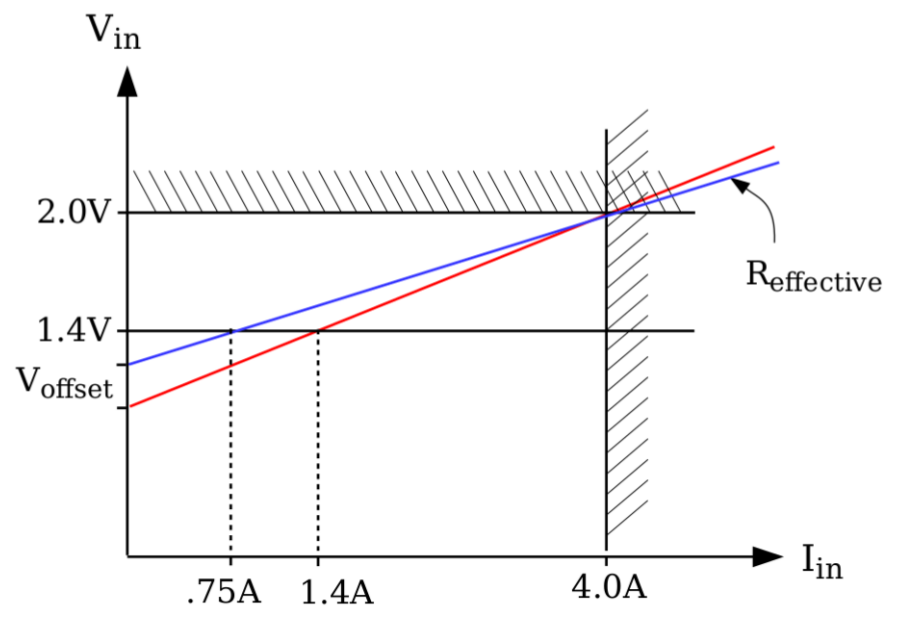
\includegraphics[scale=.3]{Immagini/VoltageVsCurrent}
\caption{Andamento tensione vs corrente del comportamento del chip. Le zone tratteggiate sono oltre i valori operativi massimi (4.0 A per la corrente e 2.0 V per la tensione), la linea orizzontale a 1.4 V è la tensione minima di lavoro, la pendenza è la resistenza efficace. Combinazioni differenti di resistenza e offset consentono di spostare il punto di lavoro.}
\label{VVC}
\end{figure}
In particolare vengono mostrati i criteri di scelta per i valori di $\mathrm{R_{eff}}$ e $\mathrm{V_{offset}}$: da una parte sarà necessario avere una corrispondenza fra la massima corrente erogabile (4.0 A) e la massima tensione (2.0 V), dall'altra si dovrà avere che la corrente corrispondente alla tensione minima di lavoro ($1.4 \V$) sia sufficiente per il funzionamento del chip.
Per garantire un buon funzionamento è indispensabile fornire la corrente con un certo margine, in modo da sopperire alle fluttuazione nei consumi.

La figura \ref{SLDOprinciple} mostra a titolo di esempio una tipica richiesta di corrente in funzione del tempo della parte digitale ed analogica.
In particolare la corrente assorbita dalla parte analogica e digitale del chip è riportata in celeste, in giallo è indicato il margine di corrente disponibile, mentre la zona rossa mostra un tipico esempio di situazione da evitare in cui la corrente richiesta dal chip è maggiore di quella disponibile
%Come si può vedere in figura \ref{VVC} I valori di $\mathrm{R_{eff}}$ e $\mathrm{V_{offset}}$ sono scelti andando a considerare i due punti di lavoro.
%Il primo è dato dalla tensione minima necessaria al funzionamento del circuito di SLDO (all'incirca $1.4 \V$), che deve essere raggiunta per un valore minimo di corrente, in modo che il chip possa funzionare correttamente.
%Questo vuol dire che per garantire il funzionamento è necessario fornire un certo margine di corrente in eccesso, poiché i consumi sono soggetti a fluttuazioni, un esempio di questo schema di lavoro è riportato in figura \ref{SLDOprinciple}.
%La corrente fornita allo SLDO è costante nel tempo, mentre quella utilizzata dal chip varia. L'aspetto che è importante sottolineare è la necessità di avere una corrente seriale che sia sempre maggiore del massimo carico in corrente, in modo da evitare fallimenti.
\begin{figure}[!htbp]
\centering
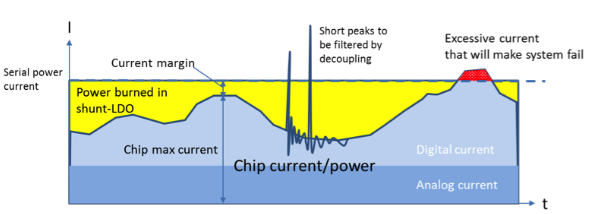
\includegraphics[scale=.5]{Immagini/ShuntRegulatorPrinciple}
\caption{Sull'asse y è riportata la corrente, mentre sulle x il tempo. La corrente assorbita dalla parte analogica e digitale del chip è riportata in celeste, in giallo è indicato il margine di corrente disponibile. La zona rossa mostra un tipico esempio di situazione da evitare in cui la corrente richiesta dal chip è maggiore di quella disponibile.}
%\caption{Sull'asse y è riportata la corrente, mentre sulle x il tempo. La corrente assorbita da parte analogica e digitale del chip è riportata in celeste, mentre in giallo è indicato il margine di corrente disponibile. Quello che si vuole evitare sono situazioni in cui la corrente richiesta dal chip è maggiore di quella discponibile, zona rossa, poiché può causare un guasto.}
\label{SLDOprinciple}
\end{figure}
%L'altro punto di interesse nel grafico è quello definito da massima tensione e massima corrente a cui è possibile alimentare il circuito. 
%Una volta sicuri che non sarà mai utilizzata una corrente maggiore del massimo per alimentare il dispositivo, si ha la sicurezza che nemmeno la tensione massima sarà raggiunta.

%% FINO A QUI ANTONIO %%
La scelta di $\mathrm{R_{eff}}$ e $\mathrm{V_{offset}}$ definisce il consumo in potenza:
\begin{equation}
\mathrm{W=I_{in}^2R_{eff}+I_{in}V_{offset}}
\end{equation}
%una $R_{eff}$ minore consente di avere minor aumento di potenza all'aumentare della corrente. 
%e dunque per un corretto funzionamento del chip è possibile utilizzare correnti minori, ovvero lasciando meno margine per le fluttuazioni, proprio perchè con $r_{eff}$ minore le fluttuazioni di corrente
La posibilità di modificare $\mathrm{R_{eff}}$ e $\mathrm{V_{offset}}$ apre alla possibilità di progettare un modo per avere diverse configurazioni, una di low-power mode e una high power mode. %Al fine di ridurre il consumo di potenza, la resistenza effettiva dello SLDO può avere un offset modificabile. 
(Low-power mode configuration, che cosa posso dire...).

L'obiettivo per il nuovo tracciatore è di aver una catena di moduli ognuno dei quali ospita quattro chip in parallelo, in figura \ref{MCM} è riportato uno schema con due moduli in serie. 
Per meglio comprendere i risvolti dati dall'utilizzo di un'alimentazione seriale con SLDO è interessante fare un esempio dei consumi di questo tipo di alimentazione. 
Prendiamo come modello la situazione in cui si ha un serie di 8 moduli con 4 chip ciascuno, assumiamo che $\mathrm{V_{offset}=0.8} \V$ e $\mathrm{R_{eff}=0.3}$ $\Omega$ per ciascun chip\footnote{$\mathrm{R_{eff}}$ del singolo SLDO è circa 0.600 $\Omega$, nel chip sono presenti due SLDO in parallelo uno per l'alimentazione della parte digitale ed uno per quella analogica. La $\mathrm{R_{eff}}$ con cui viene visto il chip è dunque la metà, 0.300 $\Omega$.}. 
Con una corrente di $\mathrm{I_{in}=2.0}$ A per chip\footnote{Che vale a dire 1 A per ciascuno dei due SLDO presenti nel chip.} ($\mathrm{I=8.0}$ A per modulo) si avrà un $\mathrm{V_{modulo}=1.4} \V$, per avere un po' di margine incrementiamo la corrente di un 20$\%$, la corrente che arriva nei moduli sarà I = 9.6 A. 

In questa situazione $\mathrm{V_{modulo}=1.52}$ V e dunque la caduta di tensione su tutta la catena formata da 8 moduli sarà pari a $12.16 \V$. Questa non è la caduta di tensione totale, va tenuto conto anche della resistenza dovuta ai cavi, in questo esempio assumiamo valga 2 $\Omega$. 
La tensione di uscita del generatore è dunque $\mathrm{V=I \cdot 2 \Omega +12.6 \V=31.8 \V}$\footnote{Circa il $60 \%$ della potenza è dissipata sui cavi, questo fatto potrebbe sembrare un pessimo traguardo, in realtà è un miglioramento rispetto alla situazione attuale, nella quale l'alimentazione è in parallelo.}.% sarebbe carino sapere la percentuale di consumo attuale
In questo sistema il generatore a monte della catena sarà limitato in corrente, mentre il limite per la tensione sarà posto leggermente maggiore a quello minimo, ad esempio 34 V. 
In questo modo la potenza che il generatore può erogare è maggiore di quella necessaria per la catena. 
Vedremo infatti, come questo sia necessario utile nel caso in cui alcuni chip smettano di funzionare. 
La potenza massima erogabile dal generatore sarà $34 \V \cdot 9.6$ $A = 326.4$ W, sottraendo la potenza dissipata sui cavi e dividendo per il numero di moduli si ottiene una potenza per modulo di $17.76$ W. Questo a fronte  di una potenza assorbita, nelle normali condizioni di lavoro, di $\mathrm{W = 4 \cdot W_{chip} = I \cdot V_{modulo} = 14.6}$ W per modulo.

\begin{figure}
\centering
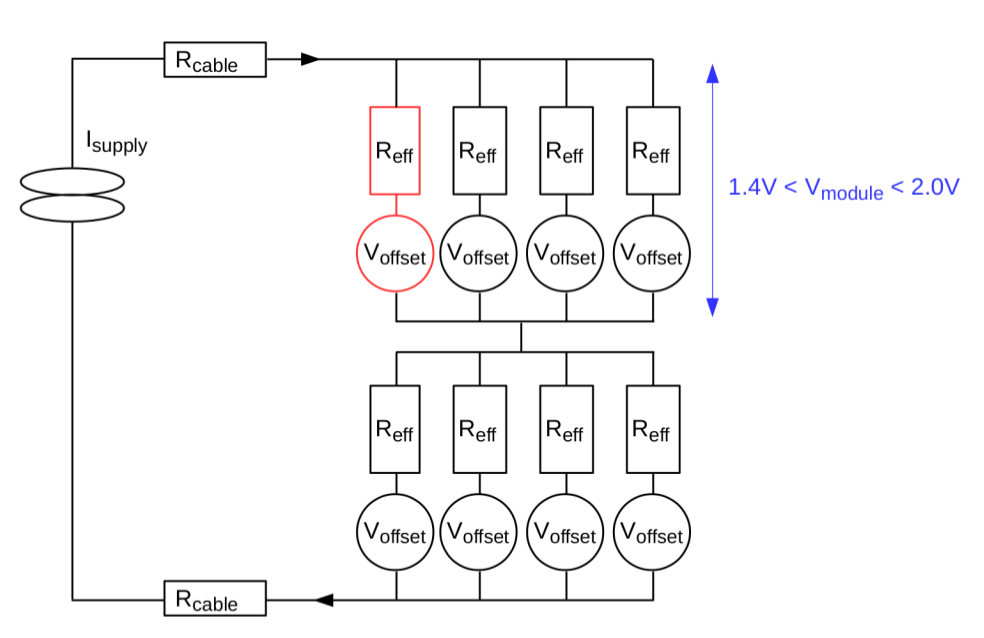
\includegraphics[scale=.3]{Immagini/MultiChipModules}
\caption{Schema di una catena seriale con moduli, ognuno formato da 4 chip. Il chip in rosso si riferisce all'ipotesi di un failure.}
\label{MCM}
\end{figure}

Vediamo a questo punto cosa accade nel caso in cui un chip in uno dei moduli sia fuori uso\footnote{Dal momento che nel chip ci sono due SLDO, in realtà lo scenario più probabile è che solo uno dei due sia danneggiato.}.
Dato che l'alimentazione è in corrente, ciascuno dei tre chip rimanenti dovrà assorbire un terzo di corrente in più, dunque la corrente per ciascun chip sarà $\mathrm{I = 9.6A / 3 = 3.2 A}$. 
Questo porta ad una caduta di tensione sul modulo $\mathrm{V_{modulo} = 3.2 A \cdot 0.3 \Omega + 0.8 V = 1.76 \V}$ e una potenza dissipata $\mathrm{W = 3 \cdot W_{chip} = 3 \cdot I \cdot V_{modulo} = 16.9}$ W, con un incremento di 2 W per il singolo modulo, che corrisponde al $13 \%$. Per la catena di 8 moduli l'incremento, invece, è di appena $1.7\%$. 
Questo causerà anche un lieve aumento della tensione erogata dal generatore, che però rimarrà al di sotto dei 34 V\footnote{Come visto alla tensione massima di  34 V il generatore riesce a distribuire una potenza di $17.76$ W per ciascun modulo.}.
 %mettere un recap con il senso di questi conti
%Lo studio dell'alimentazione seriale parte dunque dalla caratterizzazione dello SLDO. Componente che sarà poi utilizzato all'interno del chip RD53A per la generazione delle tensioni di alimentazione della parte analogica e digitale. .......continuare discorso....
Aver chiaro come il chip viene visto esternamente e quali siano i suoi consumi è importante per poter progettare al meglio il sistema di alimentazione seriale.

\section{Evoluzione design SLDO}
\begin{figure}
\centering
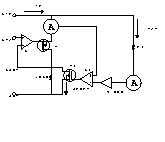
\includegraphics[scale=3.5]{Immagini/SLDObase}
\caption{Schema di principio dello SLDO.}
\label{SLDOprova}
\end{figure}

Il design del regolatore SLDO ha subito nel tempo modifiche e migliorie, fino ad arrivare all'attuale versione in tecnologia CMOS a 65 nm capace di lavorare con una corrente massima di 2A.
Partiamo da uno schema estremamente semplificato che permetta di comprendere l'idea di fondo, facendo riferimento alla figura \ref{SLDOprova}. 
Lo SLDO è alimentato in corrente $\mathrm{I_{in}}$, una frazione di questa corrente scorrerà nel ramo di R3, la indichiamo con $\mathrm{I_{ref}}$, questa sarà la corrente di riferimento all'interno dello shunt. 
La parte che agisce come regolatore di tensione è A1 + M1, A1 fa in modo di tenere la tensione sul carico uguale ad un valore di riferimento, che per ora trascuriamo come sia generato, andando ad aprire o chiudere il gate del mosfet M1 e dunque facendo scorrere più o meno corrente. 
Questo di per se causerebbe un aumento di $\mathrm{I_{ref}}$ e conseguentemente di $\mathrm{V_{in}}$ proporzionale ad R3. Nello schema è però presente un ramo in parallelo al carico, in cui la corrente che scorre è regolata da M4+A3, A3 è la parte attiva dello shunt, che fa sì che la corrente nel ramo con M1 sia 1000 volte quella che scorre in R3 andando a regolare $\mathrm{I_{shunt}}$ modificando la tensione di gate del mosfet M4. 
La corrente che scorre in M1 è dunque tenuta costante anche quando si hanno variazioni dinamiche del carico.

\begin{figure}
\centering
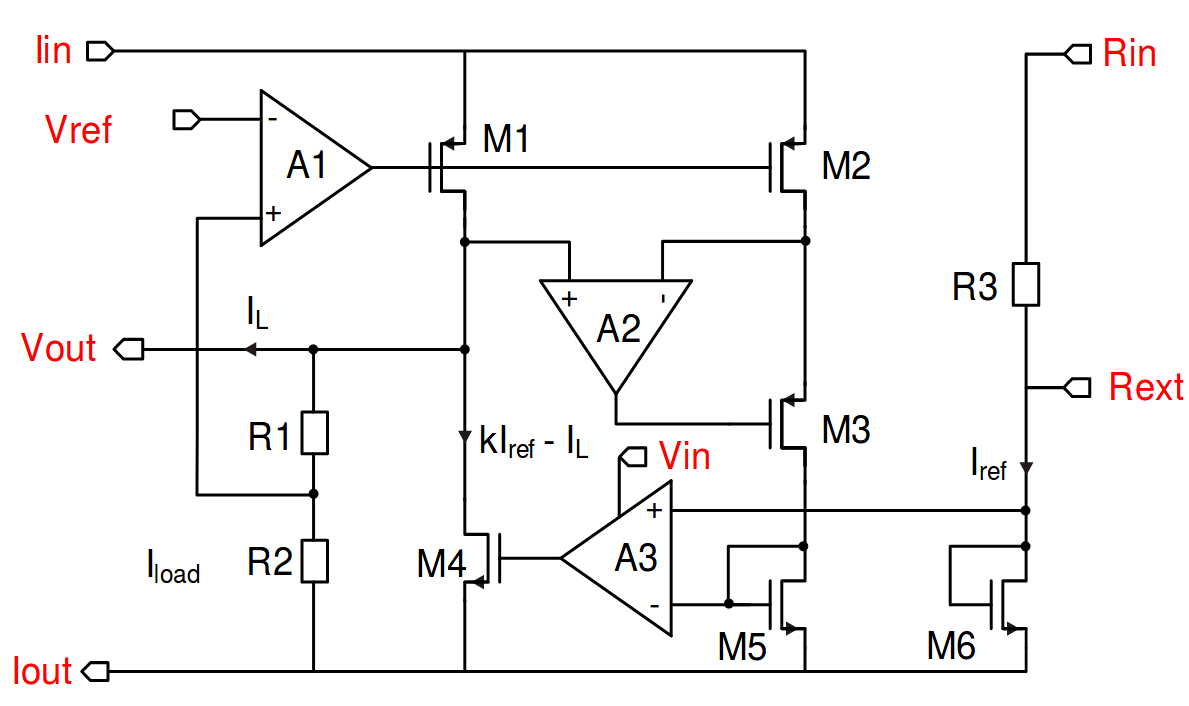
\includegraphics[scale=.3]{Immagini/SLDO5A}
\caption{Circuito semplificato dello SLDO 0.5 A.}
\label{SLDO5A}
\end{figure}

Questo primo schema permette una comprensione generale del funzionamento dell'oggetto il cui schema semplificato nella versione da $\mathrm{0.5 A}$ è riportato in figura \ref{SLDO5A}. Rispetto a quanto visto fino ad ora si hanno alcune differenze, benché l'idea generale di funzionamento rimanga la stessa. 
In questo schema il carico sta tra i pin $\mathrm{V_{out}}$ e $\mathrm{I_{out}}$ in parallelo al partitore R1+R2 (R1 e R2 sono resistenze uguali), la tensione di riferimento $\mathrm{V_{ref}}$ è confrontata con la tensione su R2 che è la metà di $V_{out}$. A3 fa un confronto tra le correnti che scorrono nel ramo di R3 ($\mathrm{I_{ref}}$) e in quello di M2 e di conseguenza regola M4. La coppia di mosfet M1-M2 è in configurazione \textit{current-mirror} e il rapporto k tra le due correnti è uguale a 1000 (dato dalle caratteristiche geometriche dei due mosfet). 
Quindi la corrente che scorre in M1 è 1000 volte $\mathrm{I_{ref}}$. Questo comportamento ci dice che esternamente lo SLDO è visto come un carico resistivo circa uguale a $\frac{R3}{k}$. A2+M3 ha lo scopo di migliorare la precisione di k, tenendo uguale la tensione a valle di M1 e M2. Il valore di R3, per quanto detto, è una importante caratteristica e la sua scelta determina la tensione nel punto di lavoro del grafico IV per una data corrente. 

Per funzionare correttamente questo circuito necessita una tensione in ingresso minima di circa $1.4V$, dunque valori di resistenza maggiori consentiranno di operare con correnti minori, con il vantaggio di consumare minor potenza\footnote{In quanto la corrente in ingresso è fissata e quella non utilizzata viene dissipata sullo shunt, che diventa un punto molto caldo}, ma con lo svantaggio di aver minor spazio per eventuali fluttuazioni del carico. 
Analogamente resistenze minori avranno l'effetto contrario, tensioni minori con correnti maggiori.
Sempre nello schematico è indicato con $\mathrm{R_{ext}}$ il punto in cui è possibile collegare una resistenza esterna in sostituzione ad R3, che è quella presente di default all'interno dello SLDO.
\begin{figure}
\centering
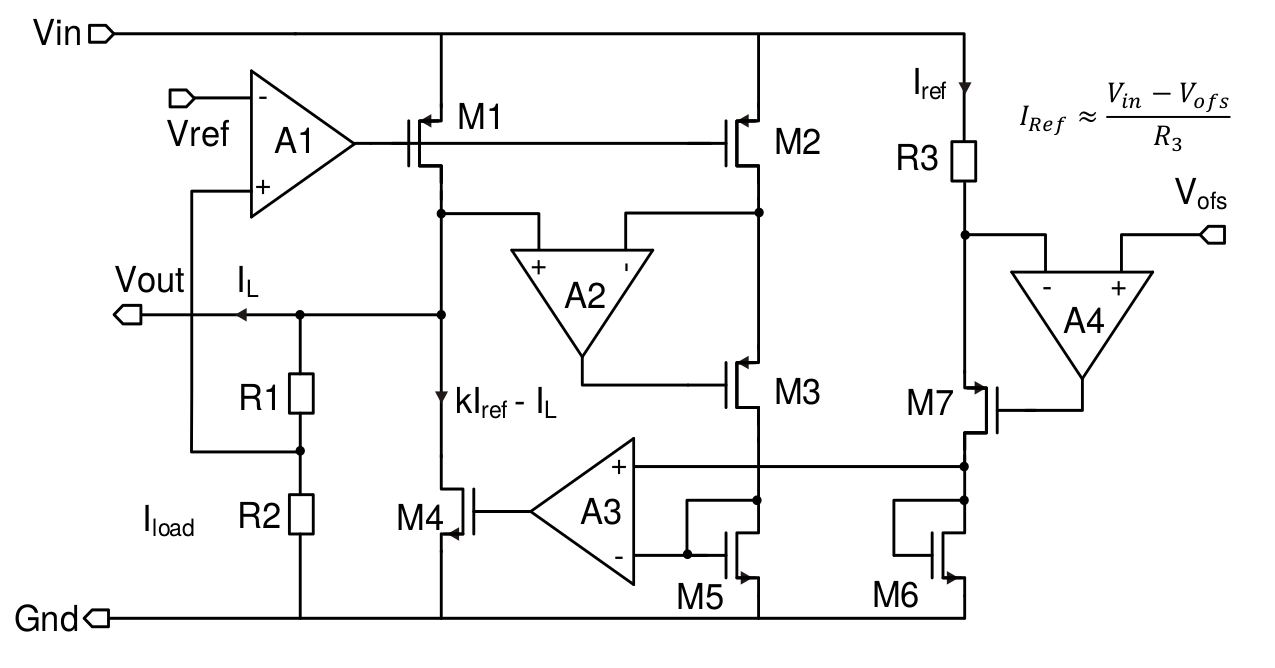
\includegraphics[scale=.3]{Immagini/SLDO2A}
\caption{Circuito semplificato dello SLDO 2A.}
\label{SLDO2A}
\end{figure}
Nel prototipo a $2A$, rispetto alla versione a $0.5A$, è presente il mosfet M7 sul ramo di R3, il cui gate è controllato da A4 (vedi figura \ref{SLDO2A}). Questo ulteriore stadio inserisce un offset di tensione al comportamento resistivo dello SLDO. In questo caso la corrente di riferimento $\mathrm{I_{ref}}$ sarà:
\begin{equation}
\mathrm{I_{ref} = \frac{V_{in} - V_{ofs}}{R_3}}
\end{equation}

\subsection{PCB}
Questa prima parte di studio del comportamento dello SLDO è stato eseguita utilizzando PCB di test nella cui parte centrale lo ShuntLDO è stato collocato e connesso con wire-bond. La PCB riportata nelle immagini è quella relativa al prototipo di ShuntLDO da 2A, figura \ref{PCBTestSLDO}. 
Sulla PCB sono presenti connettori molex per l'alimentazione, jumper di configurazione, pin per misurare varie tensioni etc. Per semplicità e chiarezza espositiva verranno introdotti solo gli elementi principali.

\begin{figure}
\centering
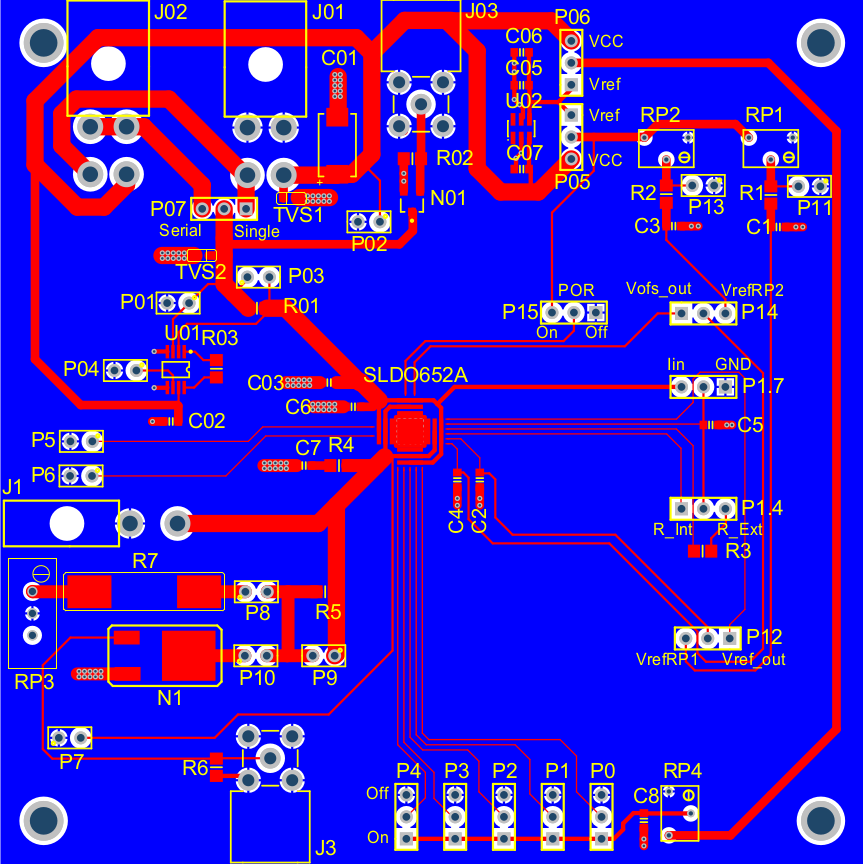
\includegraphics[scale=.3]{Immagini/chipcard}
\caption{PCB di Test per lo SLDO 2A.}
\label{PCBTestSLDO}
\end{figure}

%Aggiungere immagini reali?

L'alimentazione è fornita tramite il molex J01 la linea 1 fornisce la tensione Vcc utilizzata dal bandgap U02 per la generazione del Vref.

\section{Caratterizzazione ShuntLDO da 0.5A}
Le prime misure sono state fatte sul prototipo di SLDO da 0.5A prima del passaggio alla versione 2A. La PCB utilizzata è perciò leggermente differente da quella descritta nella sezione precedente, sebbene le funzionalità principali rimangano le stesse. Unica differenza sostanziale è la possibilità di inserire un offset regolabile al $V_{out}$, cosa che è invece possibile con la PCB dello SLDO da 2A.
Il primo studio affrontato è stato la caratterizzazione dello SLDO, utilizzando una alimentazione in corrente. Le prime misure eseguite sono state le curve tensione corrente (IV), ottenute andando a misurare la tensione in ingresso $\mathrm{V_{in}}$, quella di uscita $\mathrm{V_{out}}$ e quella di riferimento $\mathrm{V_{ref}}$ in funzione della corrente in ingresso.
\begin{figure}
\centering
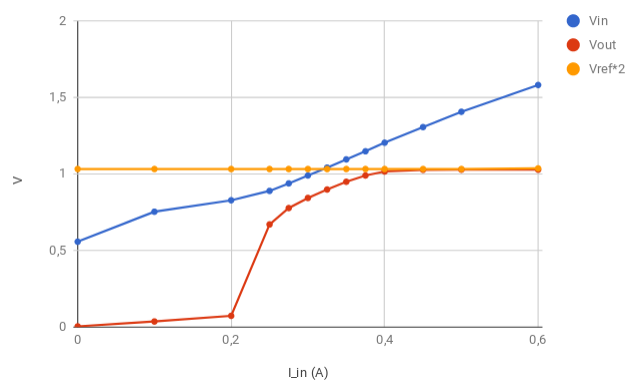
\includegraphics[scale=.5]{Immagini/provaSLDO5}
\caption{.}
\label{provaSLDO5}
\end{figure}

Le prime curve di IV sono state eseguite sullo shunt da 0.5 A in cui è possibile regolare solo $\mathrm{V_{ref}}$, in figura \ref{provaSLDO5} è riportato il grafico ottenuto andando a variare la corrente in ingresso in configurazione senza carico applicato al $\mathrm{V_{out}}$. Questa è quindi una situazione in cui tutta la corrente fornita dall'alimentazione viene assorbita dallo shunt,  prendendo l'andamento asintotico e disinteressandoci della parte iniziale del grafico, che corrisponde all'accensione dello ShuntLDO, riportiamo in tabella alcuni valori di interesse: 

\[
\begin{array}{ccccc}

\toprule
V_{ref} & V_{out} & 2 \cdot V_{ref}- V_{out} & R_{eff} & V_{offset} \\

\midrule

0.516 V & 1.028 V & 8 mV & 2.0 \Omega & 0.40 V \\

\bottomrule
\end{array}
\]
In questa prima misura non è stato applicato nessun carico al $V_out$, dunque tutta la corrente in ingresso scorre nello Shunt, questa misura ci aiuterà in un confronto successivo con situazioni in cui è presente un carico, sia statico che dinamico. 

Un'altra misura di test, che è stata eseguita con questo prototipo di shunt prima del passaggio alla versione da 2A, è un serie di due shunt entrambi con un carico resistivo di $\mathrm{4 \Omega}$. In questo caso i due ShuntLDO hanno $\mathrm{V_{ref}}$ diversi $\mathrm{V_{ref1}=0.497}$ V e $\mathrm{V_{ref2}=0.553 V}$. 
Sulla PCB è presente un bandgap la cui alimentazione può essere separata da quella dello SLDO. Il compito di questo bandgap è generare la tensione di riferimento $\mathrm{V_{ref}}$, il suo valore può essere regolato con un potenziometro, anch'esso presente sulla PCB.
Possiamo vedere a confronto il diverso comportamento nel caso in cui VCC, tensione che alimenta il bandgap sia esterna, con il caso in cui la tensione VCC sia cortocircuitata con l'ingresso di $I_{in}$ e dunque si trovi a tensione uguale a $\mathrm{V_{in}}$, figura \ref{SLDO5Serie}. In questo confronto va tenuto conto che il bandgap presente sulla scheda di test ha un regime di lavoro compreso tra  i 2 e i 18 V. 
\begin{figure}
\centering
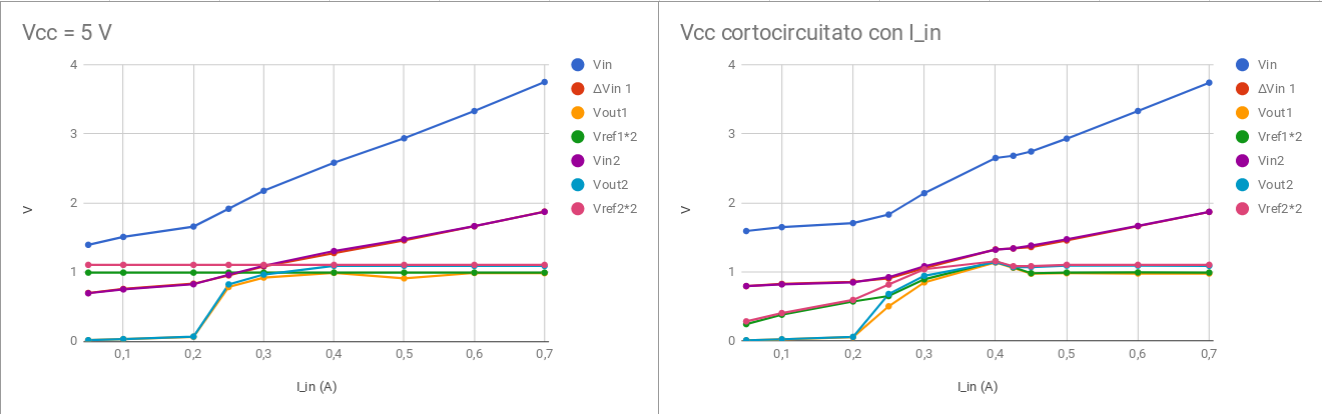
\includegraphics[scale=.3]{Immagini/SLDO5Serie}
\caption{A sinistra i bandgap sono alimentati esternamente, a destra sono alimentati tramite $V_{in}$.}
\label{SLDO5Serie}
\end{figure}
Quello che si può notare dai grafici è che fintanto che la tensione di ingresso non supera circa 1 V il bandgap non riesce a generare il giusto livello di tensione $\mathrm{V_{ref}}$ e ciò ha come conseguenza un $\mathrm{V_{out}}$ non stabile, ovvero si arriva ad una stabilità del $\mathrm{V_{out}}$ con correnti più elevate.


\subsubsection{Comportamento dinamico}
\begin{figure}
\centering
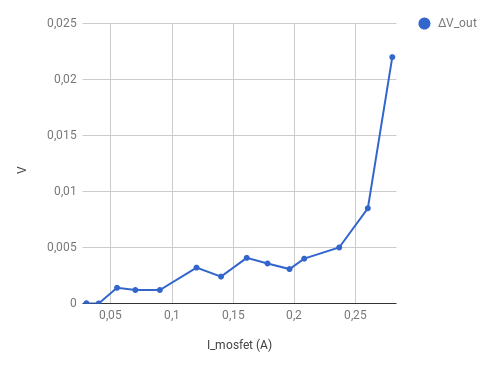
\includegraphics[scale=.5]{Immagini/SLDO5singlepulse}
\caption{Entità degli undershoot in tensione in funzione della corrente assorbita dal mosfet.}
\label{SLDO5singlepulse}
\end{figure}

Prima di passare alla versione da 2A è stata provata una situazione con carico dinamico, per poi riproporla in modo più approfondito ed esaustivo nelle sezioni successive utilizzando però il prototipo da 2A.
Nella PCB di test è presente in parallelo all'uscita di $\mathrm{V_{out}}$ un mosfet in serie ad una resistenza, il cui comportamento può essere controllato applicando una tensione dall'esterno sul gate. 
La corrente assorbita dal mosfet, può essere ricavata andando a misurare la caduta di tensione sulla resistenza. 

La prima misura di interesse è vedere quanto il $\mathrm{V_{out}}$ sia sensibile a variazioni veloci di carico. In figura \ref{SLDO5singlepulse} è riportato l'andamento dell'undershoot in funzione della corrente assorbita dal mosfet. Va tenuto presente che le misure sono state effettuate con una alimentazione in corrente $\mathrm{I_{in} = 0.5 A}$, un $\mathrm{V_{ref} \sim 0.5 V}$ e un carico resistivo su $\mathrm{V_{out}}$ di 4 $\Omega$. 
Questo perché nel momento in cui il carico dinamico più il carico statico assorbono insieme una corrente maggiore di quella totale presente in ingresso il sistema va in crisi. Gli effetti visibili in situazioni in cui $\mathrm{I_{mosfet} + I_{load} > I_{in}}$ non hanno perciò direttamente a che vedere con il comportamento dello SLDO. 
Si può vedere dal grafico \ref{SLDO5singlepulse} come gli undershoot rimangano inferiori a 10 mV fin tanto che $\mathrm{I_{mosfet}}$ rimane sotto gli 0.250 A, valore oltre cui $\mathrm{I_{mosfet} + I_{load} > I_{in}}$\footnote{$\mathrm{I_{load}}$ è la corrente che scorre nel carico resistivo, in questo caso $\mathrm{I_{load} = \dfrac{V_{out}}{R} = 0.250 A}$}. 

Lo stesso test può essere eseguito mettendo due SLDO in serie ed andando a variare dinamicamente il carico di uno dei due, verificando se esternamente queste variazioni siano visibili, e quindi se influenzino l'altro elemento della catena seriale. 
Dal momento che l'interesse maggiore è per il prototipo a 2 A questo tipo di misura non è stato riportato nel caso dello SLDO da 0.5A, in quanto lo scopo di questa prima parte è quello di introdurre un certo tipo di approccio e  prendere confidenza con gli argomenti trattati.

\section{ShuntLDO 2A}
%\begin{figure}
%\centering
%\includegraphics[scale=.3]{Immagini/PCB2A}
%\caption{.}
%\label{PCB2A}
%\end{figure}
Rispetto a quanto visto in precedenza, nella versione da 2 A è possibile gestire anche l'offset attraverso un potenziometro RP2 che va ad agire sulla tensione in uscita generata dal bangap, la stessa che viene utilizzata per generare $\mathrm{V_{ref}}$ regolando un secondo potenziometro RP1. 

\section{Comportamento statico}
La parte di caratterizzazione statica è di nuovo eseguita andando a variare la corrente di alimentazione in ingresso e al contempo misurando $\mathrm{V_{out}}$, $\mathrm{V_{ref}}$ e $\mathrm{V_{in}}$, figura \ref{SLDO2Astatic}.

\begin{figure}
\centering
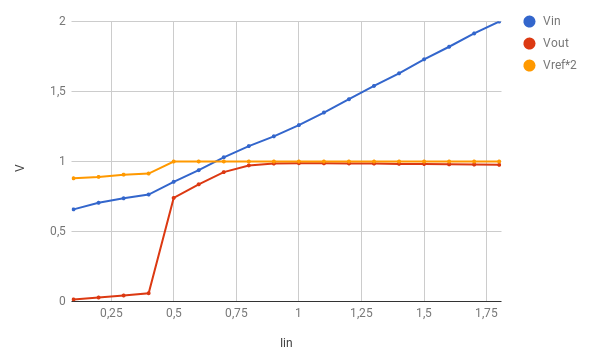
\includegraphics[scale=.5]{Immagini/SLDO2Astatic}
\caption{.}
\label{SLDO2Astatic}
\end{figure}

Questo andamento è stato ottenuto ponendo\footnote{Per selezionare il valore voluto è necessario regolare il potenziometro RP1 che si trova in serie al bandgap sulla PBC.} $\mathrm{V_{ref} = 0.5} V$ e applicando un carico resistivo di 1 $\Omega$ a $\mathrm{V_{out}}$. Il bandgap è alimentato esternamente con una tensione di 5 V. 
Come si vede dal grafico \ref{SLDO2Astatic} delle IV $\mathrm{V_{ref}}$ non è costante nella parte iniziale, questo può essere dovuto al fatto che nella fase in cui lo shunt LDO non è attivo si ha uno scorrimento di corrente nel ramo di $\mathrm{V_{ref}}$, ciò causa una maggiore caduta di tensione sul potenziometro e quindi una minore tensione all'ingresso di A4. 
Idealmente, nel ramo di $\mathrm{V_{ref}}$ dovrebbe scorrere una corrente molto piccola in regime di lavoro\footnote{Questo perché nello SLDO il $\mathrm{V_{ref}}$ è in ingresso al comparatore A1 e viene confrontato con una tensione che sarà circa uguale in una situazione di equilibrio. La corrente che scorre tra ingresso + e - sarà piccola, poiché il comparatore in ingresso ha una grossa resistenza.}, mentre al momento dell'accensione, all'ingresso di A1 si ha una notevole differenza tra + e -, e quindi scorrerà una corrente maggiore, questo è causa di una variazione del $\mathrm{V_{ref}}$. Di seguito riportiamo in tabella i valori che si riferiscono al grafico \ref{SLDO2Astatic}: 

\[
\begin{array}{ccccc}

\toprule
V_{ref} & V_{out} & 2 \cdot V_{ref}- V_{out} & R_{eff} & V_{offset} \\

\midrule

0.500 V & 0.980 V & 20 mV & 0.880 \Omega & 0.40 V \\

\bottomrule
\end{array}
\]

\subsection{Differenze tra GND PCB e GND SLDO}
Prima di procedere oltre è interessante fare alcune riflessioni per porre attenzione su un aspetto che influenza le misure. 
Tutte le tensioni misurate, come per esempio il $\mathrm{V_{out}}$, sono eseguite utilizzando pin sulla PCB. Questo vuol dire che, per esempio, quando viene misurato $\mathrm{V_{out}}$ la tensione letta sull'oscilloscopio o attraverso i multimetri è la differenza di tensione tra il pin di $\mathrm{V_{out}}$ sulla PCB e la terra (GND) della medesima. Dal momento che questi punti di misura sono collegati al $\mathrm{V_{out}}$ dello ShuntLDO attraverso wire bond si introduce una resistenza, che causa una caduta di tensione. L'entità di questa caduta di tensione dipende dalla resistenza dei wire bond e dalla corrente, dunque nel caso di una caratterizzazione con carico statico si presenta come un offset, mentre nel caso di carico dinamico varia al variare della corrente. 
I wire bond si presentano con tante resistenze in parallelo, perciò il valore di questa resistenza dipende dal numero di wire bond eseguiti. Dunque maggiore sarà il numero di questi ultimi minore sarà il valore della resistenza equivalente e dunque minore sarà l'effetto su $\mathrm{V_{out}}$. Questo problema è riportato schematicamente in figura \ref{Ground}.

\begin{figure}
\centering
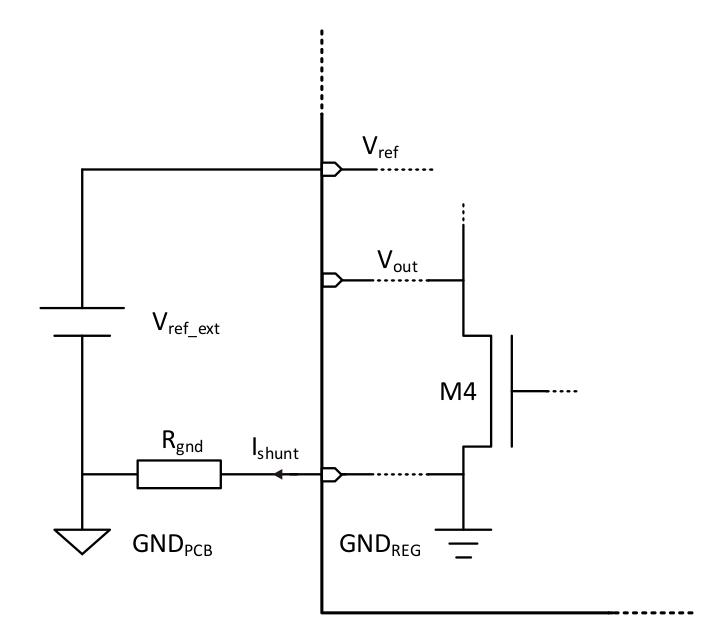
\includegraphics[scale=.3]{Immagini/Ground}
\caption{Differenze tra $\mathrm{GND_{PCB}}$ e $\mathrm{GND_{REG}}$ nella configurazione ShuntLDO, causate dalla corrente di shunt.}
\label{Ground}
\end{figure}

Ricapitolando, nella configurazione di ShuntLDO una frazione della corrente in ingresso scorre attraverso il transistor di shunt (M4), questa corrente confluisce nella linea di terra del regolatore $\mathrm{GND_{REG}}$ e da qui, attraverso i wire bond è collegata alla terra della PCB ($\mathrm{GND_{PCB}}$). La resistenza di questa linea, schematizzata in figura con una resistenza $\mathrm{R_{GND}}$, è la causa della differenza in tensione tra la terra della PCB e dello Shunt. Questo spiega anche il fatto che $\mathrm{V_{ref_ext}}$ sia leggermente maggiore di $\mathrm{V_{out}}$. Infatti  $\mathrm{V_{ref_ext}}$ è esterno allo shunt e dunque l'effettiva tensione di riferimento vista dallo shunt è minore. Il $\mathrm{V_{out}}$ realmente prodotto dallo ShuntLDO sarà:
\begin{equation}
\mathrm{V_{out} = 2 \cdot V_{ref} = 2 \cdot ( V_{ref {\_} ext} - I_{shunt} \cdot R_{gnd} )}
\end{equation}

Questo effetto è appena visibile in figura \ref{SLDO2Astatic}, dove all'aumentare della corrente $\mathrm{V_{out}}$ si ha una lieve flessione della tensione in uscita. Facendo un fit lineare dei punti si ottiene una pendenza di - 0.015 $\Omega$. 
La pendenza ottenuta del fit non è unicamente data dai wire bond ma ha un contributo aggiuntivo dato dalla resistenza delle piste e dei connettori. 
Una misura più precisa può essere eseguita sfruttando i pin $\mathrm{V_{out{\_}Sense}}$ e $\mathrm{I_{out {\_} Sense}}$, rispettivamente indicati sulla PCB con P5 e P6. 
Questi due pin di monitoraggio sono collegati rispettivamente al $\mathrm{V_{out}}$ del regolatore e al GND sempre del regolatore. 
Essendo piste in cui non scorre corrente, l'effetto resistivo di wire bond è eliminato ed è possibile misurare il valore di tensione del GND locale.

\begin{figure}
\centering
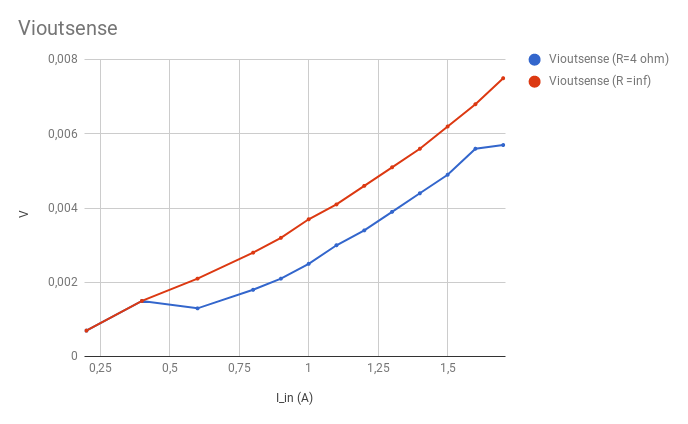
\includegraphics[scale=.4]{Immagini/Viout}
\caption{Andamento della tensione del GND dello shunt rispetto al GND della PCB al variare della corrente di alimentazione del circuito.}
\label{VioutSense}
\end{figure}

Si è proceduto a misurare il valore di tensione sul pin $\mathrm{I_{out{\_}Sense}}$ al variare della corrente di alimentazione $\mathrm{I_{in}}$. 
La misura è stata eseguita per due diversi valori di carico statico $4 \Omega$ e $\infty$, con il valore infinito si intende la configurazione in cui il carico è assente e dunque il circuito tra $\mathrm{V_{out}}$ e GND è aperto, presentandosi di fatto come una resistenza infinita. 
In figura \ref{VioutSense} è possibile vedere come le due diverse configurazioni di carico influenzino la misura con un offset. 
Infatti nei due casi la pendenza è la stessa e dà un'indicazione del valore resistivo R dei wire bond, l'offset invece rispecchia il fatto che lo spostamento di tensione è dato dalla corrente che scorre verso il GND del chip, che nel caso in cui il carico richieda più corrente diminuisce. Ad esempio a 1 A con i carico resistivo da 4 $\Omega$ la corrente che effettivamente scorre verso GND nello shunt è 0.75 A (questo nel caso $\mathrm{V_{out} = 1 V}$).

\[
\begin{array}{cccc}

\toprule
\mathrm{R_{rossa}}  & \mathrm{R_{blu}} & \mathrm{offset_{rosso}} & \mathrm{offset_{blu}} \\

\midrule

\mathrm{4 m} \Omega & \mathrm{4 m}\Omega & \mathrm{-1 mV}  & \mathrm{-2 mV} \\

\bottomrule
\end{array}
\]

Il valore di questa resistenza è molto piccolo e come detto dipende in prima approssimazione dal numero di wire bond. Fintanto che lo ShuntLDO è utilizzato come circuito a se stante su una PCB di test questo aspetto risulta secondario, in quanto non ci sono problemi di spazio e si può utilizzare un gran numero di connessioni per ridurre al minimo differenze tra $\mathrm{GND_{PCB}}$ e $\mathrm{GND_{REG}}$.   

  
\subsection{Offset}
Come detto in precedenza nella versione da 2 A è possibile regolare esternamente il $\mathrm{V_{offset}}$. 
Una tensione di offset alta consente di raggiungere il punto di lavoro prima, cioè con un minor consumo di corrente, mentre un valore di $\mathrm{V_{offset}}$ basso ha l'effetto contrario. Questo effetto lo si può verificare andando a misurare la tensione di output $\mathrm{V_{out}}$ per diversi valori di $\mathrm{V_{offset}}$ al variare di $\mathrm{I_{in}}$.

\begin{figure}
\centering
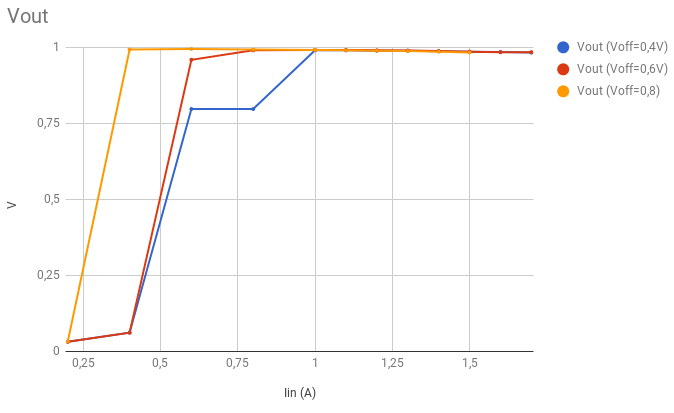
\includegraphics[scale=.4]{Immagini/VoutVsVoffset}
\caption{Andamento di $\mathrm{V_{out}}$ al variare della corrente in ingresso per differenti valori di $\mathrm{V_{offset}}$.}
\label{VoutVsVoffset}
\end{figure}

Andando a misurare $\mathrm{V_{in}}$ al variare della corrente in ingresso è possibile ricavare, con un fit lineare nella regione di funzionamento del circuito, l'intercetta con l'asse y che corrisponde all'offset. 
Questi valori sono riportati nella tabella seguente:

\begin{figure}
\centering
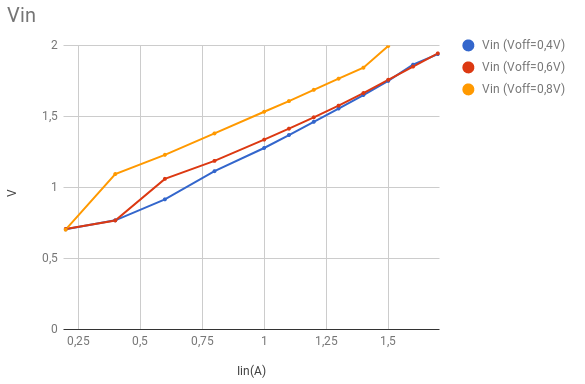
\includegraphics[scale=.4]{Immagini/VinVsVoffset}
\caption{Andamento di $\mathrm{V_{in}}$ al variare della corrente in ingresso per differenti valori di $\mathrm{V_{offset}}$.}
\label{VinVsVoffset}
\end{figure}

\[
\begin{array}{ccc}

\toprule
\mathrm{Offset 0.4 V} & \mathrm{Offset 0.6 V} & \mathrm{Offset 0.8 V} \\

\midrule

0.352 V & 0.539 V & 0.756 V \\

\bottomrule
\end{array}
\]

Come si può vedere il valore effettivo è sempre leggermente minore. Questo è un risultato che troveremo anche più avanti nelle misure eseguite sullo ShuntLDO presente all'interno del chip RD53A. 

\section{Comportamento dinamico}

\begin{figure}
\centering
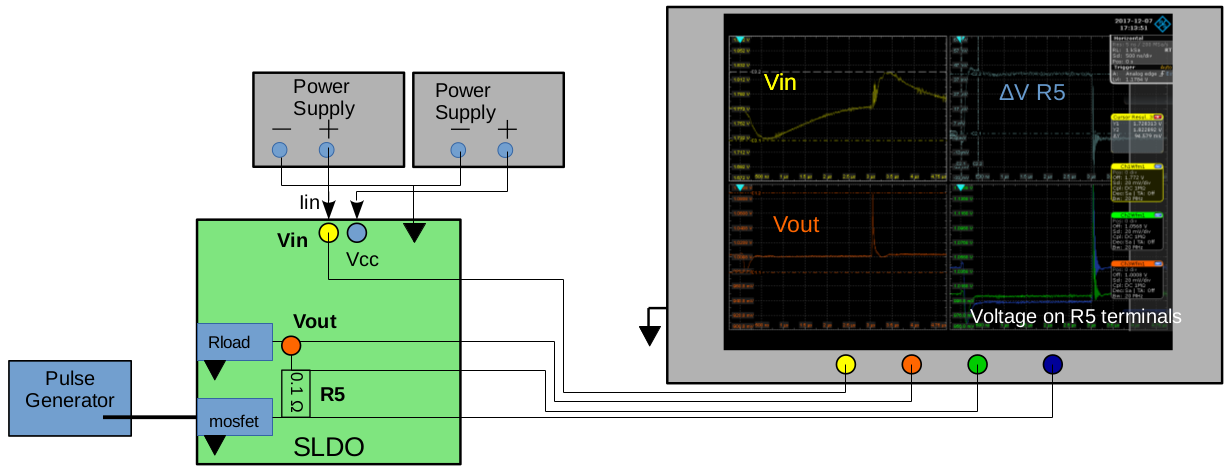
\includegraphics[scale=.3]{Immagini/SetupScheme}
\caption{Schema del setup per lo studio del comportamento dinamico dello SLDO.}
\label{Setupscheme}
\end{figure}

Oltre alla caratterizzazione statica è interessante studiare il comportamento dello SLDO in risposta ad una variazione dinamica del carico, andando a focalizzare l'attenzione sulla velocità dello shunt nel riequilibrare il consumo in corrente. La risposta dinamica è dipendente da fattori quali il punto di lavoro a cui si trova lo SLDO, il tempo in cui avviene la variazione di carico e l'entità di tale variazione. 
Il circuito è alimentato tramite un generatore di corrente a 1.5 A e $\mathrm{Vref=0.5 A}$, dunque ci aspettiamo una tensione all'uscita di 1 V. Al fine di introdurre un carico dinamico, in parallelo al carico statico, è presente un mosfet in serie ad una resistenza R5 di $0.1 \Omega$. 
La corrente assorbita dal mosfet, indicata con $\mathrm{I_{mosfet}}$ sarà ricavata misurando la caduta di tensione sulla resistenza. 
Il mosfet è pilotato tramite un generatore di impulsi. A seconda dell'ampiezza del segnale inviato al gate del mosfet c'è una maggiore o minore corrente che scorre tra drain e source. 
Il setup di queste misure è rappresentato schematicamente in figura \ref{Setupscheme}, sulla sinistra vi è la PCB in verde, mentre in grigio sono riportati gli alimentatori, sulla destra vi è l'oscilloscopio con cui sono misurate la tensione in ingresso $\mathrm{V_{in}}$\footnote{L'alimentazione dello SLDO è comunque in corrente.}, rappresentata in giallo, la tensione in uscita $\mathrm{V_{out}}$, in arancione, e le tensioni agli estremi della resistenza R5. Infine sulla sinistra della PCB collegato al gate del mosfet è presente un generatore di impulsi. 
Per quanto riguarda la durata dell'impulso da mandare al gate del mosfet si è scelto di tenere fronte di salita e discesa ben distanti in modo da osservare separatamente gli effetti dovuti al fronte di salita da quelli di discesa. 
In una situazione in cui il carico del regolatore è il chip le variazioni sarebbero di minor durata rispetto alla lunghezza dell'impulso utilizzato in queste misure, però lo scopo di queste misure è vedere gli effetti che si hanno al passaggio da un certo consumo di corrente ad uno maggiore e viceversa. 
Un impulso di breve durata avrebbe il problema di sovrapporre questi due effetti, non permettendo di valutarne l'effettiva entità, in quanto i contributi sono opposti e su tempi brevi si sovrappongono cancellandosi.
In queste misure l'attenzione sarà focalizzata su variazioni di $\mathrm{V_{in}}$ e $\mathrm{V_{out}}$ in ampiezza e sul tempo di recupero al variare di $\mathrm{I_{mosfet}}$ per una data $\mathrm{R_{load}}$.

L'introduzione di questo carico, in parallelo alla resistenza connessa a $\mathrm{V_{out}}$, è possibile posizionando un jumper sul pin P10 della PCB. Già dalle prime misure con l'oscilloscopio è visibile come che l'utilizzo del mosfet come carico dinamico non sia esente da problematiche che vanno ad alterare i segnali, rendendo difficile una corretta interpretazione. 
Prendendo a riferimento la figura \ref{TransientTest} si nota innanzitutto un'asimmetria nelle variazioni di $\mathrm{V_{out}}$, posto in basso a sinistra e di colore arancione, mentre in $\mathrm{V_{in}}$, posto in alto a sinistra e di colore giallo, la risposta è simmetrica. In azzurro è riportata la differenza tra le tensioni misurate ai capi di R5, che invece sono riportate in blu e in verde, da cui è possibile calcolare la corrente che scorre tra Drain e Source del mosfet. 
Inoltre sono visibili delle oscillazioni in corrispondenza del momento in cui il mosfet si spegne e smette di assorbire corrente. Questo comportamento si riflette su $\mathrm{V_{out}}$, ed è quindi all'origine dell'asimmetria. Questo aspetto è stato approfondito prima di procedere a misure della risposta dinamica nelle varie combinazioni $\mathrm{I_{mosfet}}$-$\mathrm{R_{load}}$, al fine di capire a cosa fosse dovuto, sospettando un contributo del mosfet non trascurabile.
In questa prima fase l'impulso utilizzato ha le seguenti caratteristiche: frequenza 50 Hz, durata 3 $\mu$ s, durata del fronte di salita 40 ns.
\begin{figure}
\centering
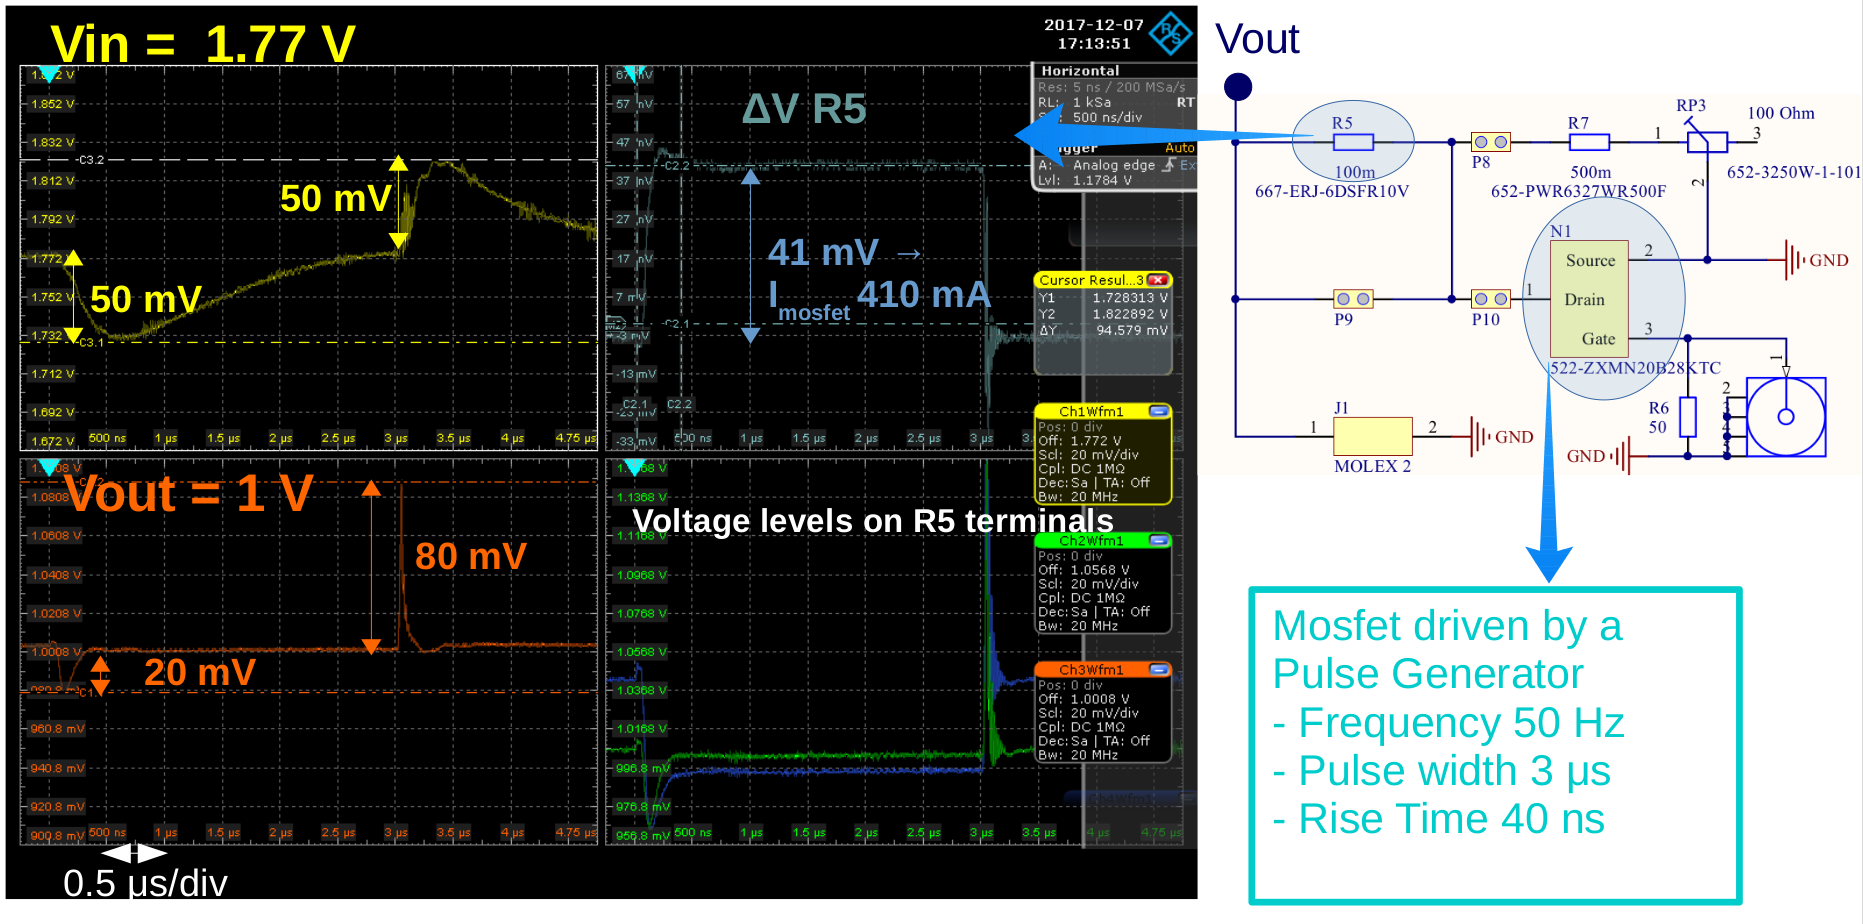
\includegraphics[scale=.2]{Immagini/TransientTest}
\caption{.}
\label{TransientTest}
\end{figure}

\subsubsection{Contributo mosfet}
Per esaminare il comportamento del mosfet in risposta all'impulso mandato sul gate si è proceduto ad isolare questa parte del circuito dal resto della PCB andando a connettere sul pin P10 (connesso al drain del mosfet) una resistenza in serie ad una batteria stilo. La batteria ricopre il ruolo di $\mathrm{V_{out}}$, mentre la resistenza è necessaria alla misura delle correnti che scorrono nel mosfet. La resistenza utilizzata è $R=2.7 \Omega$. 

\begin{figure}
\centering
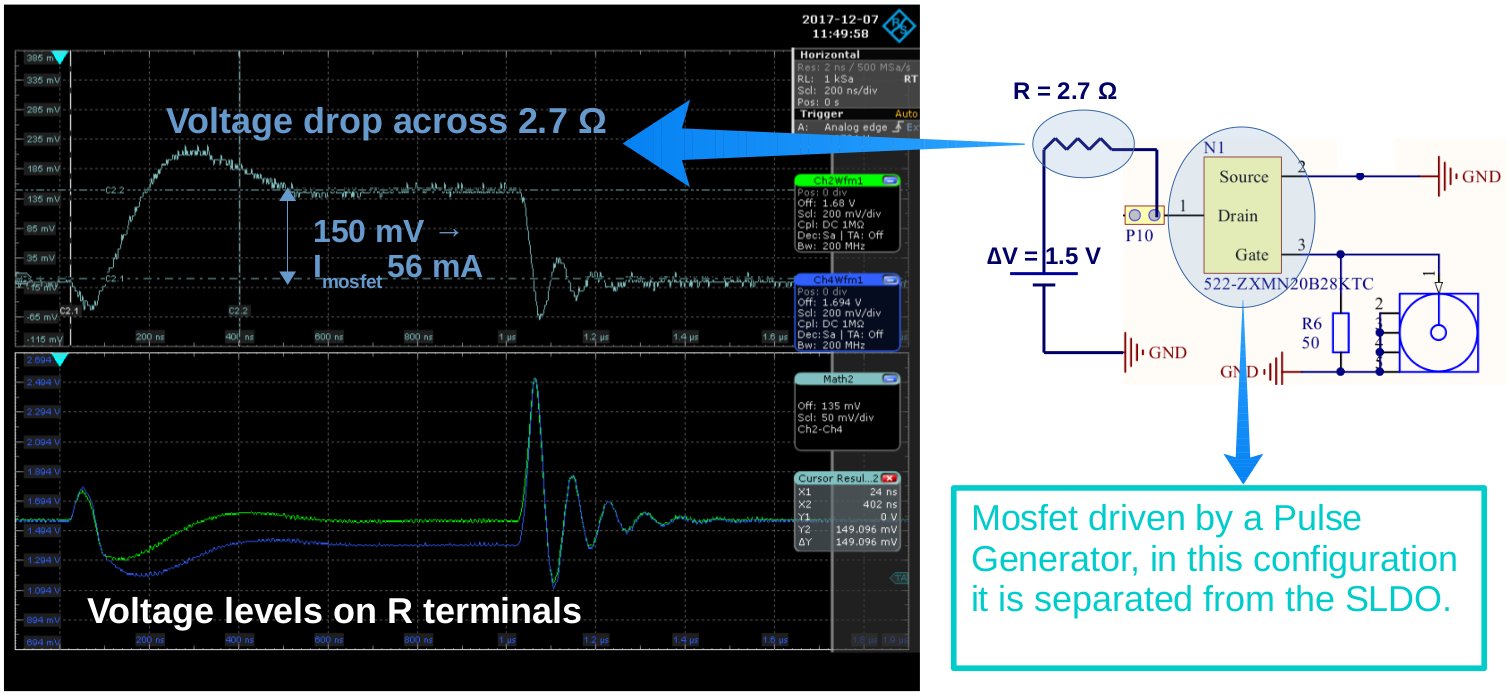
\includegraphics[scale=.3]{Immagini/MosfetBehaviour}
\caption{.}
\label{MosfetBehaviour}
\end{figure}

\begin{figure}
\centering
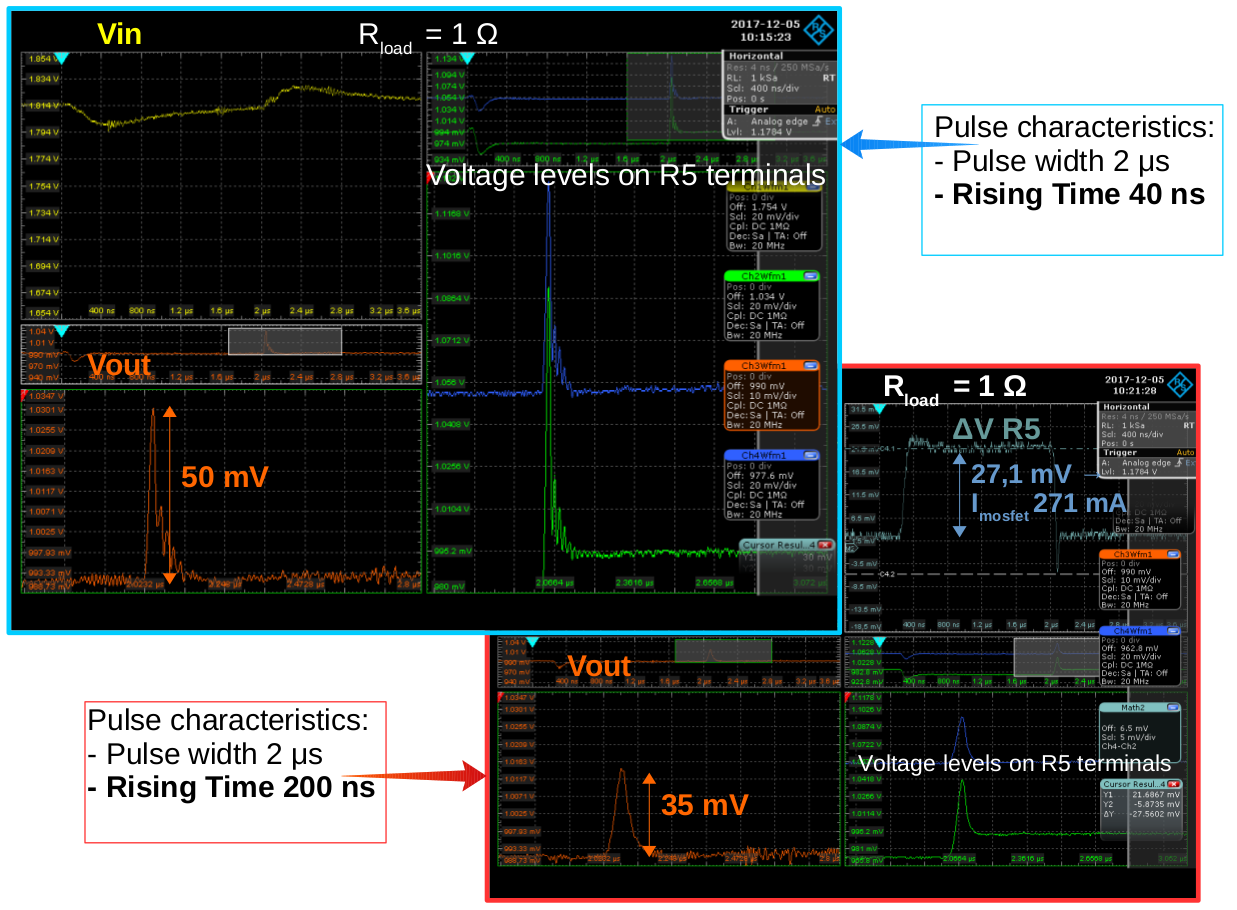
\includegraphics[scale=.3]{Immagini/RiseTime}
\caption{.}
\label{RiseTime}
\end{figure}

Come è possibile vedere dalla figura \ref{MosfetBehaviour}, le oscillazioni sono presenti anche una volta isolato il mosfet, segno che sono generate da quest'ultimo nel momento in cui il canale che collega drain e source si interrompe, inoltre il fronte di salita è circa 100 ns e non 40 ns come ci aspetteremmo da un mosfet ideale con risposta istantanea. Andando a esaminare la documentazione del mosfet presente sulla PCB 
%footnote{ZXMN20B28KTC http://www.mouser.com/ds/2/115/ZXMN20B28K-94822.pdf
si può verificare che effettivamente il tempo di "accensione" è superiore a 40 ns (Turn-on rise time 76,9 ns) e inoltre sono presenti capacità in ingresso di $\mathrm{358 pF}$. Tutto questo rende impossibile vedere la risposta dello SLDO a segnali più veloci della risposta del mosfet, per questo motivo le misure successive sono state prese impostando un tempo di salita del segnale del generatore di impulsi di 200 ns.
In figura \ref{RiseTime} è visibile come la situazione precedente, in cui l'impulso ha un tempo di salita di 40 ns, migliora visibilmente passando a 200 ns, in questo modo quello che viene simulato all'uscita dello ShuntLDO è un variazione di carico più lenta ma il cui comportamento è affetto in modo minore dalle caratteristiche del mosfet. 

\subsubsection{Misure}
A questo punto si è proceduto con le misure della tensione di ingresso $\mathrm{V_{in}}$ e di uscita $\mathrm{V_{out}}$ per tre differenti valori di $\mathrm{R_{load}}$ al variare di $\mathrm{I_{mosfet}}$. I valori di $\mathrm{R_load}$ scelti sono stati $1 \Omega$, $2.1 \Omega$ e $4 \Omega$, e dato che $\mathrm{V_{out}=1V}$ in termini di correnti  $\mathrm{I_{load}}$ corrispondono rispettivamente 1 A, 0.475 A e 0.250 A. A questo punto per vari valori di $\mathrm{I_{mosfet}}$ sono stati misurate le variazioni in ampiezza e il tempo di recupero di $\mathrm{V_{in}}$ e $\mathrm{V_{out}}$.

Una prima differenza che si nota è il differente tempo di recupero tra $\mathrm{V_{in}}$ e $\mathrm{V_{out}}$, molto più lungo dell'ordine dei $\mu$s e dipendente dall'entità di $\mathrm{I_{mosfet}}$ per il primo mentre per il secondo ha durata di circa 300 ns indipendentemente dal valore di $\mathrm{I_{mosfet}}$. 
Questo è dovuto al fatto che il riequilibrio della tensione di ingresso dipende anche dal generatore esterno le cui variazioni sono più lente.
Va ricordato che lo SLDO è alimentato in corrente con 1.5 A, dunque nel momento in cui $\mathrm{I_{load}+I_{mosfet}}$ raggiungono valori vicini o addirittura superiori  a $\mathrm{I_{in}}$ si ha un crollo della tensione in ingresso e del $\mathrm{V_{out}}$. Questo è un effetto aspettato in quanto si sta chiedendo allo SLDO di fornire una corrente superiore a quella a sua disposizione.


Per ciascun valore di $\mathrm{R_{load}}$, come detto in precedenza, è stata fatta variare la corrente assorbita dal mosfet $\mathrm{I_{mosfet}}$ ed è stato misurato l'effetto di undershoot e overshoot sulle tensioni di $\mathrm{V_{out}}$ e $\mathrm{V_{in}}$. 
% Con corrente totale si intende la somma di quella assorbita dal mosfet e dalla resistenza di carico.
Le misure eseguite prendono in considerazioni anche situazioni in cui la variazione del consumo in corrente eccede l'intervallo fisico di operatività del chip. 
Misure in cui la variazione del carico è il doppio del valore statico hanno interesse nell'ottica di quello che può succedere al momento dell'accensione del chip, le cui variazioni di consumo in regime di lavoro di norma non superano i 500 mA.(controllare) 
Come detto in precedenza gli impulsi utilizzati presentano una durata che consente di differenziare tra effetti dovuti al fronte di salita e effetti dati dal fronte di discesa dell'impulso. 
I primi risultati riportano gli undershoot della tensione di uscita a cui è applicato il carico, riferendosi ai grafici in figura \ref{VoutUnd} sono riportati i valori assoluti di tali variazioni in funzione della corrente che scorre nel mosfet (sinistra) e della corrente totale (destra), la corrente totale è somma di quella assorbita dal carico e dal mosfet. 
\begin{figure}
\centering
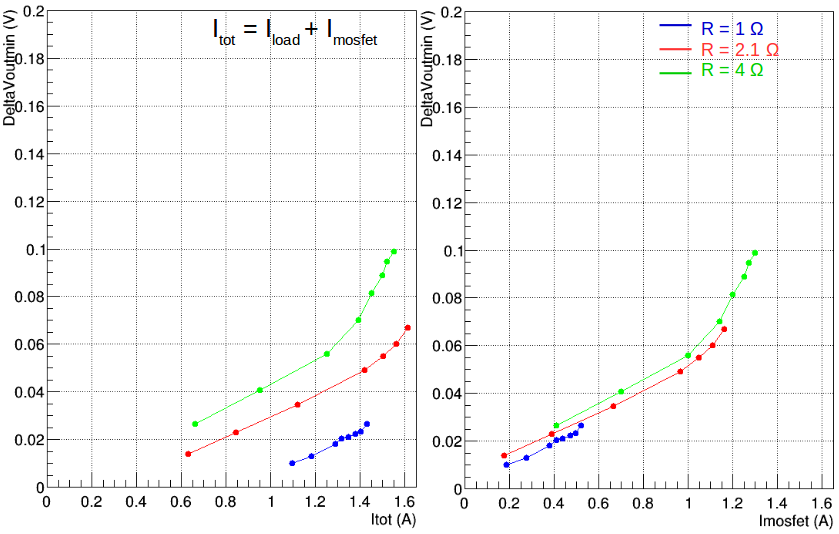
\includegraphics[scale=.44]{Immagini/VoutUnd}
\caption{Grafici che riportano l'entità dell'undershoot del $\mathrm{V_{out}}$ in funzione della corrente totale, grafico di sinistra, e della corrente del mosfet, grafico di destra.}
\label{VoutUnd}
\end{figure}
\begin{figure}
\centering
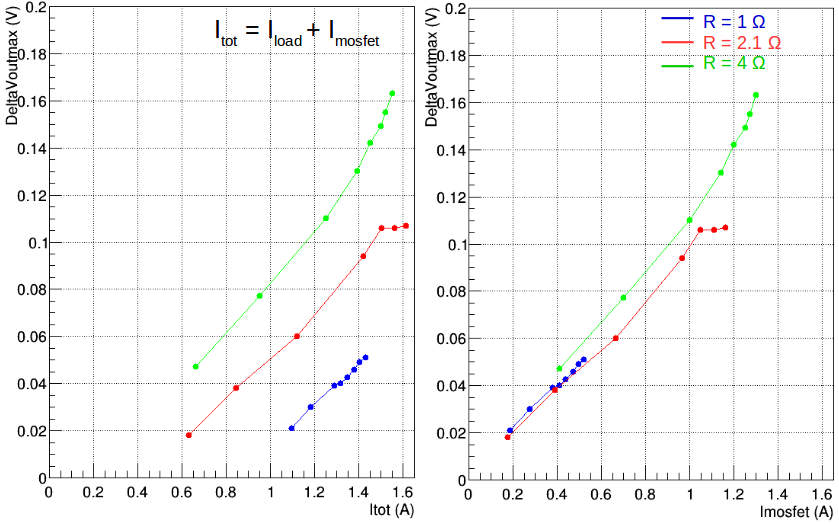
\includegraphics[scale=.44]{Immagini/VoutOver}
\caption{Grafici che riportano l'entità dell'overshoot del $\mathrm{V_{out}}$ in funzione della corrente totale, grafico di sinistra, e della corrente del mosfet, grafico di destra.}
\label{VoutOver}
\end{figure}
In blu sono riportati le misure ottenute con un carico resistivo di 1 $\Omega$, in rosso 2.1 $\Omega$ e in verde 4 $\Omega$. 
Come si può vedere dal grafico di destra  vi è una dipendenza della variazione di $\mathrm{V_{out}}$ da $\mathrm{I_{mosfet}}$, in quanto le tre curve seguono lo stesso andamento, indipendente dal valore della resistenza.
Inoltre, riferendosi ad un intervallo di variazioni di corrente verosimili per il chip, si hanno variazioni relativamente piccole di $\mathrm{V_{out}}$. Con $\mathrm{I_{mosfet}= 0.4 }$ A il $\mathrm{\Delta V_{out} \simeq 20mV}$.
Lo stesso comportamento è visibile nei grafici di figura \ref{VoutOver}, dove è riportata l'entità delle variazioni di $\mathrm{V_{out}}$ a seguito dello spegnimento del mosfet, cioè l'effetto che si ha sul fronte di discesa dell'impulso. 
Nell'esaminare questi andamenti va ricordato che la corrente in ingresso al circuito è 1.5 A, quindi punti per i quali si ha una $\mathrm{I_{tot}}$ vicina o superiore a questo valore sono ottenuti in una situazione in cui lo SLDO è impossibilitato a compiere il suo lavoro. 
La corrente che passa in R3 è un millesimo di quella che scorre nel in ramo in cui si ha carico e shunt.

Come per il $\mathrm{V_{out}}$ è stato misurato l'undershoot e l'overshoot della tensione in ingresso $\mathrm{V_{in}}$. I grafici degli undershoot sono riportati in figura \ref{VinUnd}, quelli riguardanti gli overshoot in figura \ref{VinOver}. 
In entrambi i casi la variazione della tensione in ingresso dipende sia dalla variazione di corrente $\mathrm{I_{mosfet}}$ che dalla corrente fissa $\mathrm{I_{load}}$. 
Per valori elevati di $\mathrm{I_{mosfet}}$ la tensione in ingresso inizia ad oscillare, con periodi di qualche $\mu$s. Questo comportamento è dovuto al generatore utilizzato, in particolare l'alimentazione in corrente è stata ottenuta utilizzando un generatore di tensione e limitando la corrente in uscita. 
Nel momento in cui si ha una variazione di carico molto veloce che, come abbiamo visto, provoca un abbassamento di $\mathrm{V_{out}}$ si ha una piccola ripercussione sulla tensione di ingresso. 
Dato che il generatore è di tensione limitato in corrente al fine di tenere costante $\mathrm{I_{in}}$ avrà un abbassamento di tensione, che però ha tempi più lunghi rispetto a quelli con cui lo ShuntLDO riesce a riequilibrare $\mathrm{V_{out}}$. Il comportamento oscillatorio di $\mathrm{V_{in}}$ che compare quando $\mathrm{I_{tot}}$ è  intorno al valore massimo, cioè $\mathrm{I_{in}}$, ha permesso di constatare come fluttuazioni della tensione in ingresso non influiscano sulla tensione generata dal regolatore. Questo può essere visto bene utilizzando l'oscilloscopio, in figura \ref{DipVoutVin} è mostrato uno screenshoot in cui è riportato in giallo l'andamento della tensione in ingresso in funzione del tempo, e in arancione la tensione di $\mathrm{V_{out}}$. Si nota come le scale di tempo di recupero siano differenti, alcuni $\mu$s per $\mathrm{V_{in}}$ e circa 300 ns per $\mathrm{V_{out}}$.

\begin{figure}
\centering
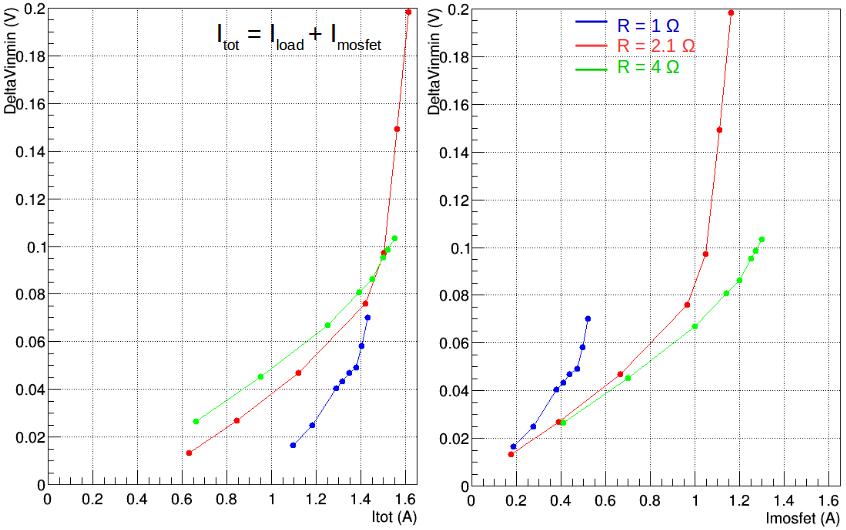
\includegraphics[scale=.45]{Immagini/VinUnd}
\caption{Grafici che riportano l'entità dell'undershoot del $\mathrm{V_{in}}$ in funzione della corrente totale, grafico di sinistra, e della corrente del mosfet, grafico di destra.}
\label{VinUnd}
\end{figure}
\begin{figure}
\centering
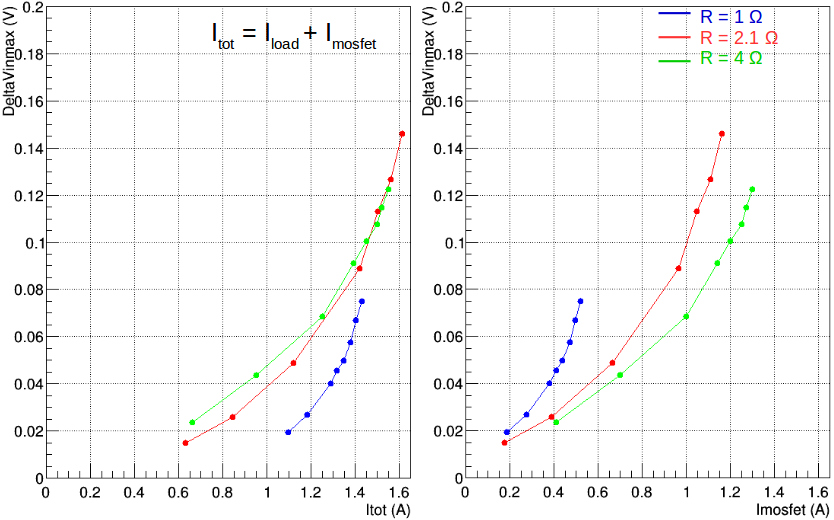
\includegraphics[scale=.45]{Immagini/VinOver}
\caption{Grafici che riportano l'entità dell'undershoot del $\mathrm{V_{in}}$ in funzione della corrente totale, grafico di sinistra, e della corrente del mosfet, grafico di destra.}
\label{VinOver}
\end{figure}

\newpage
\begin{figure}
\centering
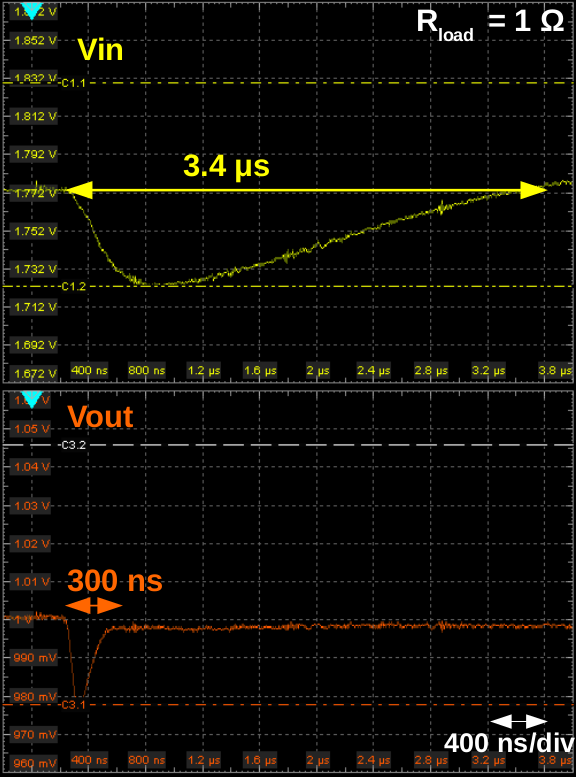
\includegraphics[scale=.35]{Immagini/DipendenzaVoutdaVin}
\caption{Differenze nei tempi di recupero tra $\mathrm{V_{out}}$, in giallo, e $\mathrm{V_{out}}$, in arancione.}
\label{DipVoutVin}
\end{figure}

\subsubsection{Serie di due SLDO}
Eventuali oscillazioni della tensione in ingresso causerebbero oscillazioni di tensione in tutta la catena di moduli, per questo motivo è importante che esse non si ripercuotano sul $\mathrm{V_{out}}$. 
Per verificare questo aspetto si è proceduto con il monitorare la tensione di uscita di uno SLDO messo in serie con un secondo a cui è stato applicato un carico variabile, tramite l'utilizzo del mosfet, come nelle misure precedenti, in figura \ref{SLDOserie} sono affiancati uno schema del setup (sinistra) e la foto dei due SLDO in serie (destra). 
Il serie di due SLDO, entrambi con un carico statico di 4 $\Omega$, è stato alimentato con una corrente in ingresso di 1.5 A. Sul secondo SLDO è stato collegato l'impulsatore che regola l'assorbimento di corrente  da parte del mosfet. 
Monitorando all'oscilloscopio la tensione di $\mathrm{V_{out}}$ di entrambi e il $\mathrm{V_{in}}$ del primo shunt della catena (quello con solo carico statico) è stato possibile verificare come le fluttuazioni di tensione non influenzino la generazione della tensione di $\mathrm{V_{out}}$. In figura \ref{ScreenSerie} si può vedere come, nonostante il secondo SLDO sia al limite il primo non ne risente nel generare $\mathrm{V_{out}}$. 
Questo campionamento dei segnali fatto con l'oscilloscopio è stato ottenuto con una $\mathrm{I_{mosfet}}$ di 1.2 A e quindi con una $\mathrm{I_{tot}}$ di circa 1.45 A, molto vicino al limite di 1.5 A. 
\begin{figure}[h!]
\centering
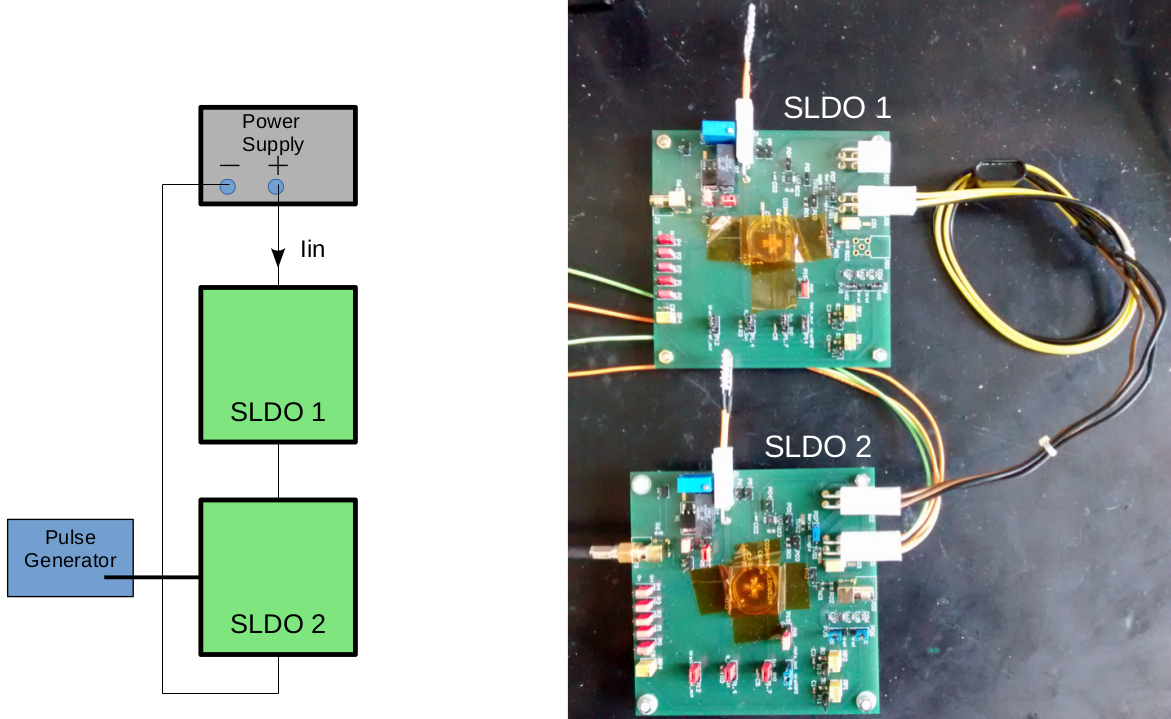
\includegraphics[scale=.30]{Immagini/SLDOserie}
\caption{Sulla destra foto dei due SLDO in serie di cui a sinistra è riportato uno schema delle connessioni con generatore e impulsatore.}
\label{SLDOserie}
\end{figure}
\begin{figure}[h!]
\centering
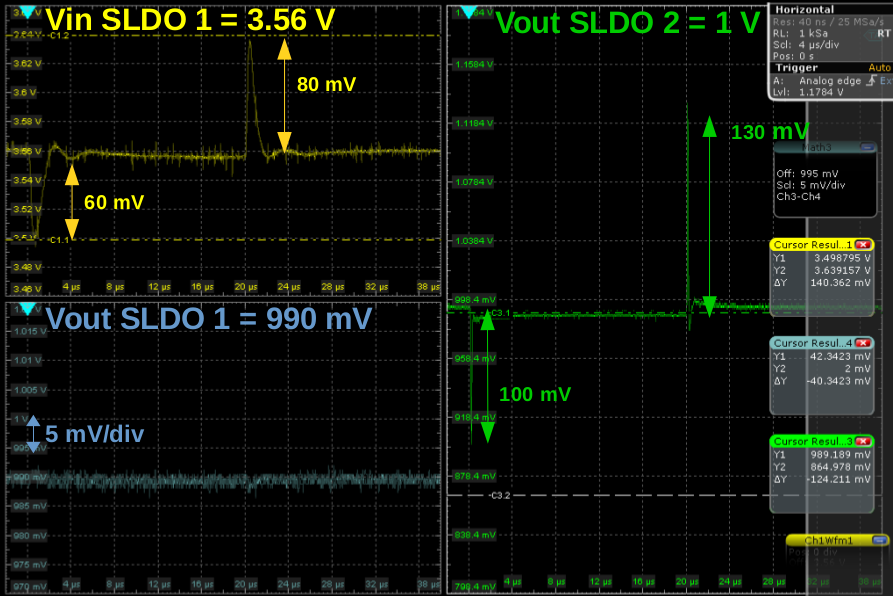
\includegraphics[scale=.32]{Immagini/ScreenSerie}
\caption{Schermata dell'oscilloscopio in cui è riportata in giallo la tensione in ingresso al primo SLDO della catena,  in celeste la tensione di $\mathrm{V_{out}}$ sempre dello SLDO1 e in verde la tensione di $\mathrm{V_{out}}$ dello SLDO2 su cui è applicato il carico dinamico. Le fluttuazioni in tensione originate dalla variazione di carico sullo SLDO 2 si ripercuotono sul $\mathrm{V_{in}}$ dello SLDO1 (giallo) ma non sulla tensione da esso generata (celeste).}
\label{ScreenSerie}
\end{figure}
In verde è riportato l'andamento del $\mathrm{V_{out}}$ del secondo SLDO, che infatti ha importanti undershoot e overshoot, i quali causano come visto in precedenza, fluttuazioni della tensione in ingresso. 
La tensione di ingresso dello SLDO2 non è altro che la terra della PCB su cui si trova lo SLDO1, fluttuazioni di questa si ripercuotono e sono visibili in ingresso. 
Il risultato importante è come niente di tutto questo sia visibile sul $\mathrm{V_{out}}$ del primo SLDO.
